\section*{Lecture 16}

\subsection*{1.} Let
\[ 
y_1(t) = e^{t}, \,  y_2(t) = e^{2t}, \, -\infty < t < \infty
.\]
Sketch $y_2(t)$ as a function of $y_1(t)$ in the $y_1y_2$-plane.
\bigbreak
We can quickly see that:
\[ 
y_2(t) = e^{2t} = \left( e^{t} \right)^2 = \left( y_1(t) \right)^2
.\]
Therefore we have:
\[ 
y_2 = y_1^2
.\]
This can be plotted as:
\begin{figure} [ht]
  \centering
  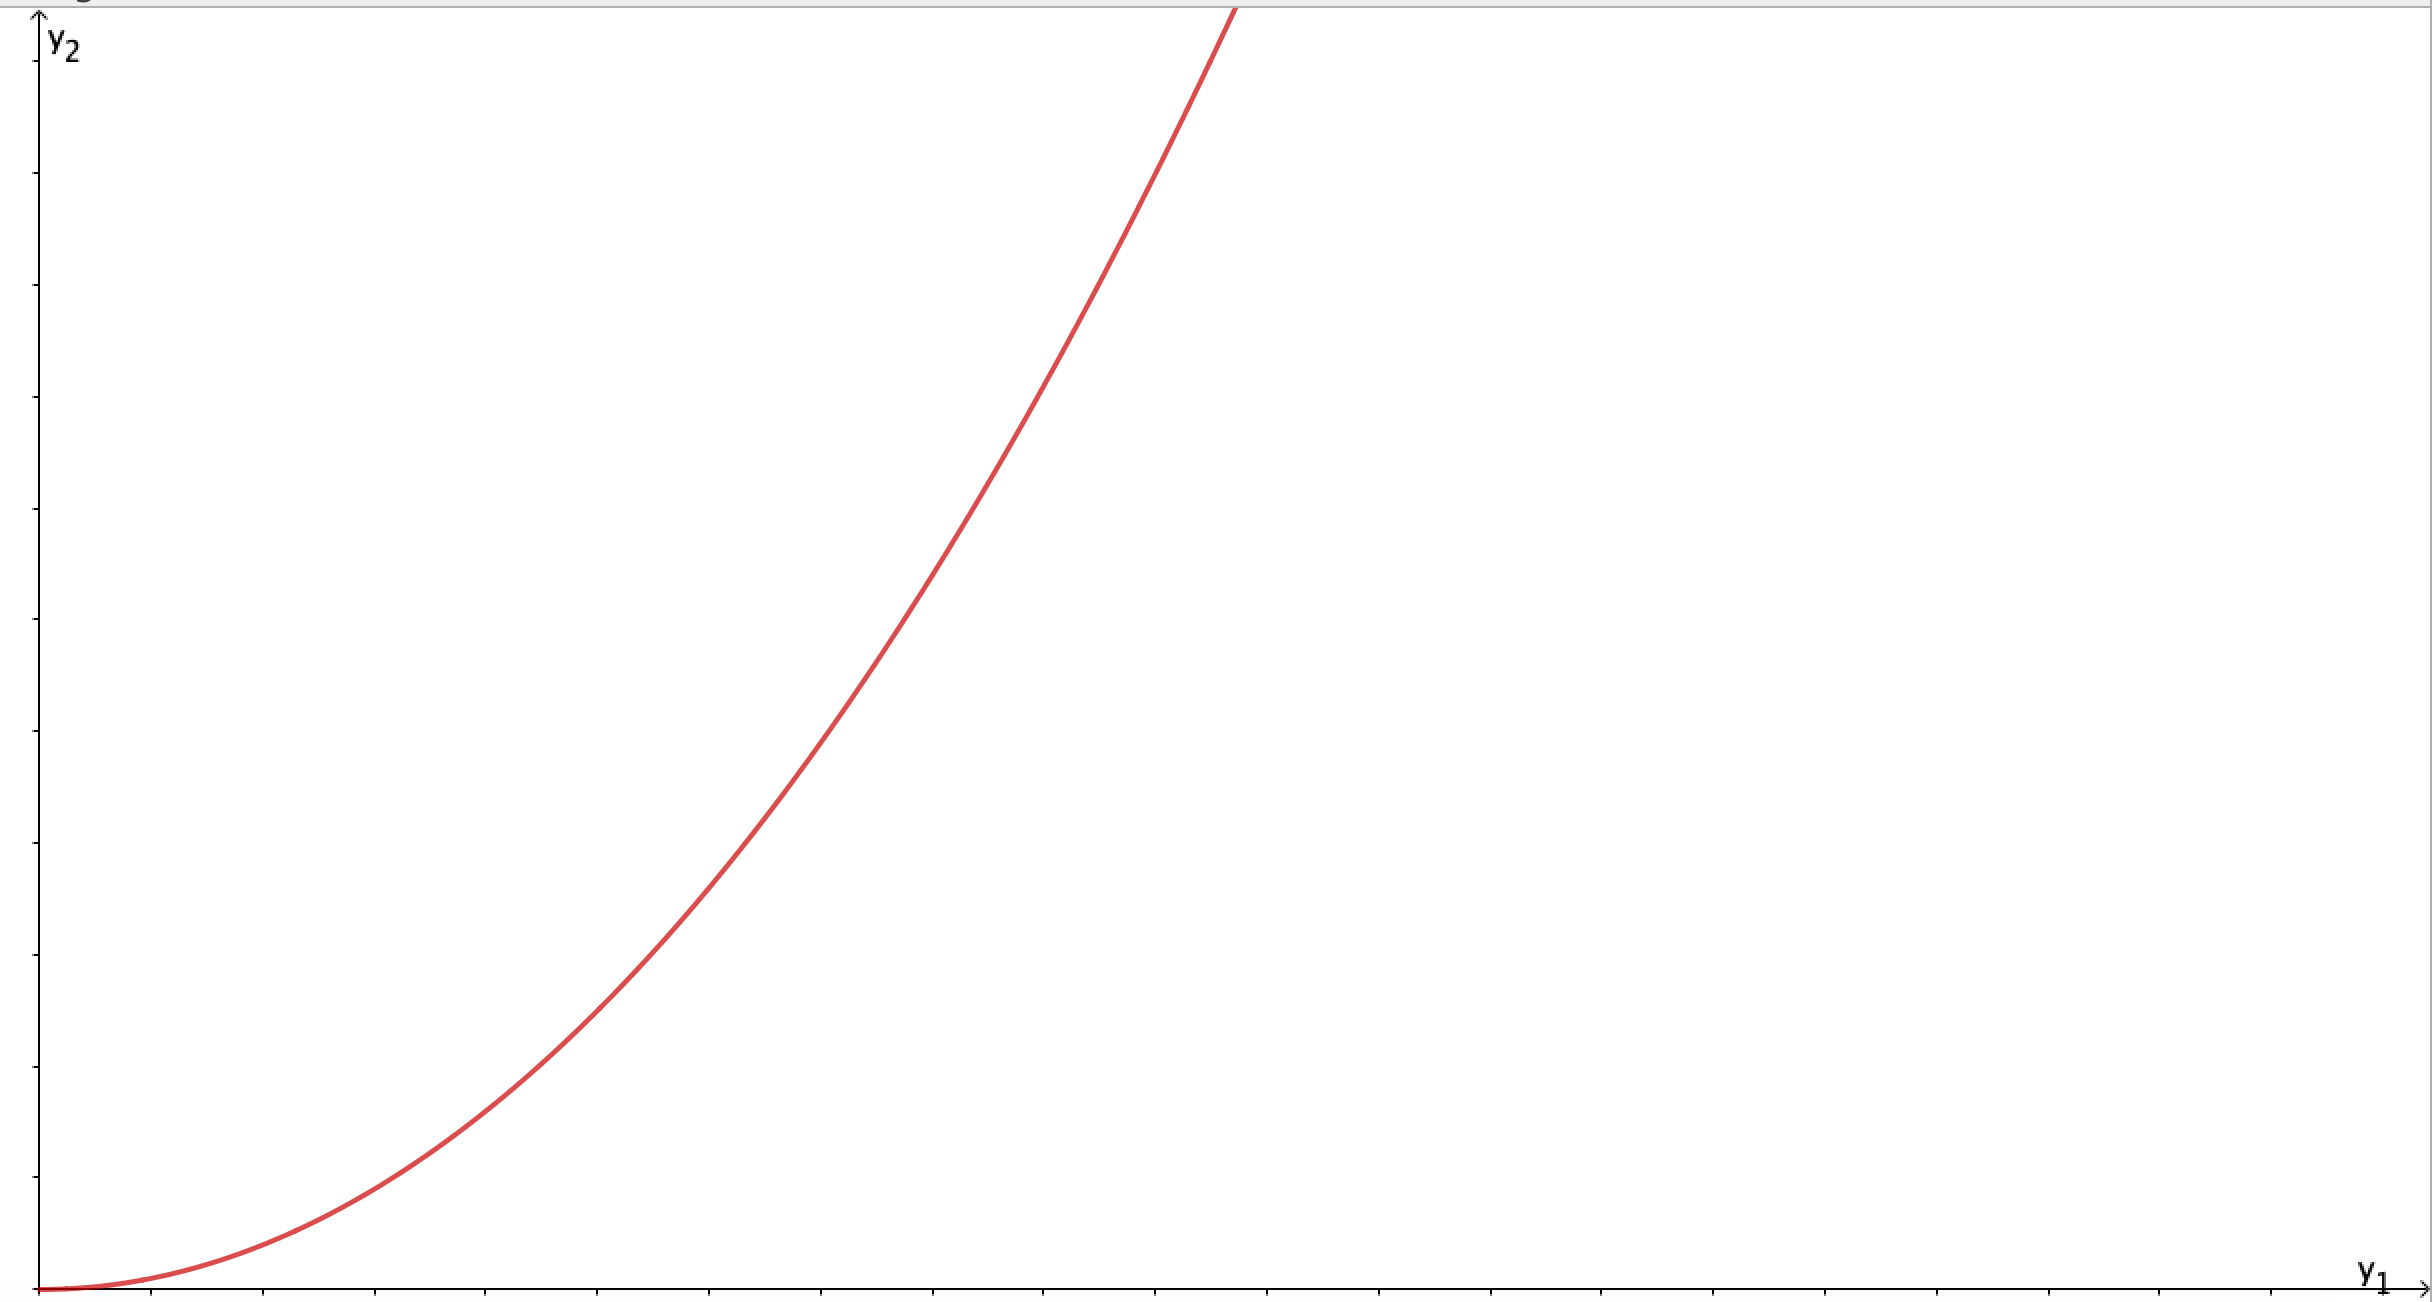
\includegraphics[width=0.5\linewidth]{./figures/e16_1.png}
  \caption{}
  \label{fig:e16_1}
\end{figure}


\subsection*{2.} Let
\[ 
y_1(t) = e^{t}, y_2(t) = t, -\infty < t < \infty
.\]
Sketch $y_2(t)$ as a function of $y_1(t)$ in the $y_1y_2$-plane.
\bigbreak
This time we realize that:
\[ 
y_2(t) = t = \ln e^{t} = \ln y_1(t)
.\]
Therefore we have:
\[ 
y_2 = \ln y_1
.\]
Which can be plotted as:
\begin{figure} [ht]
  \centering
  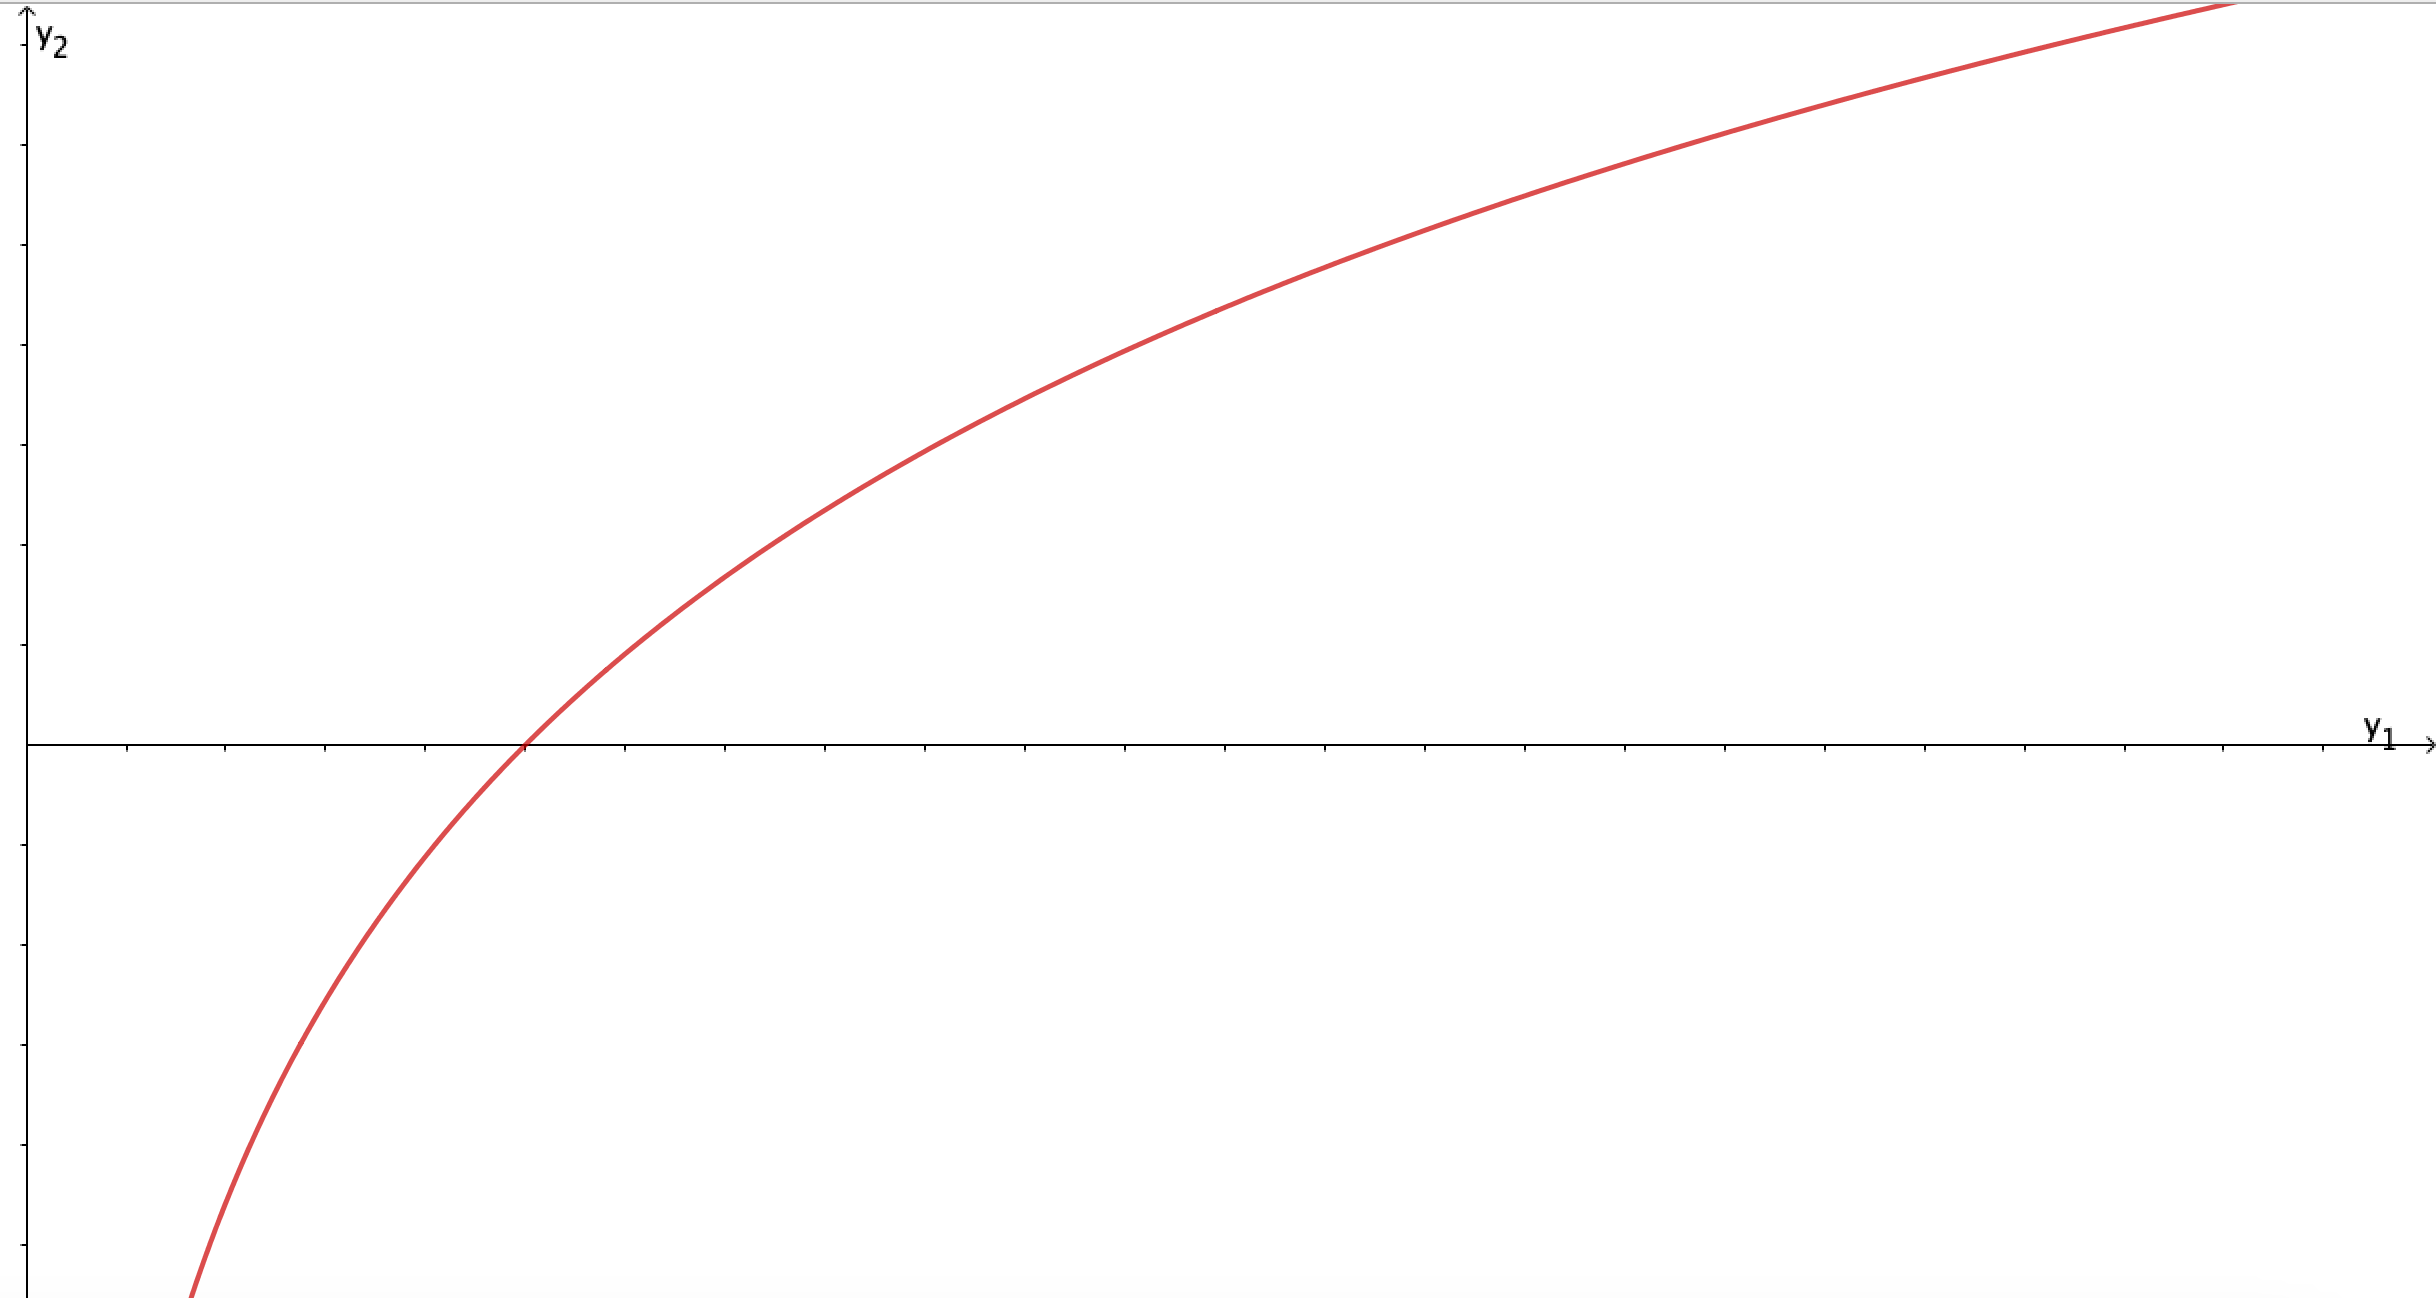
\includegraphics[width=0.5\linewidth]{./figures/e16_2.png}
  \caption{}
  \label{fig:e16_2}
\end{figure}


\subsection*{3.} Let
\[ 
y_1(t) = e^{t} + 1, y_2(t) = e^{t} + e^{2t}, -\infty < t < \infty 
.\]
Sketch $y_2(t)$ as as a function of $y_1(t)$ in the $y_1y_2$-plane.
\bigbreak
This time we must do some more work in order to write $y_2(t)$ in terms of $y_1(t)$. First we see that:
\[ 
y_1(t) - 1 = e^{t}
.\]
Therefore we can write $y_2(t)$ in terms of $y_1(t)$ as:
\[ 
y_2(t) = e^{t} + e^{2t} = y_1(t) - 1 + \left( y_1(t) - 1 \right)^2
.\]
Which can be plottes as:
\begin{figure} [ht]
  \centering
  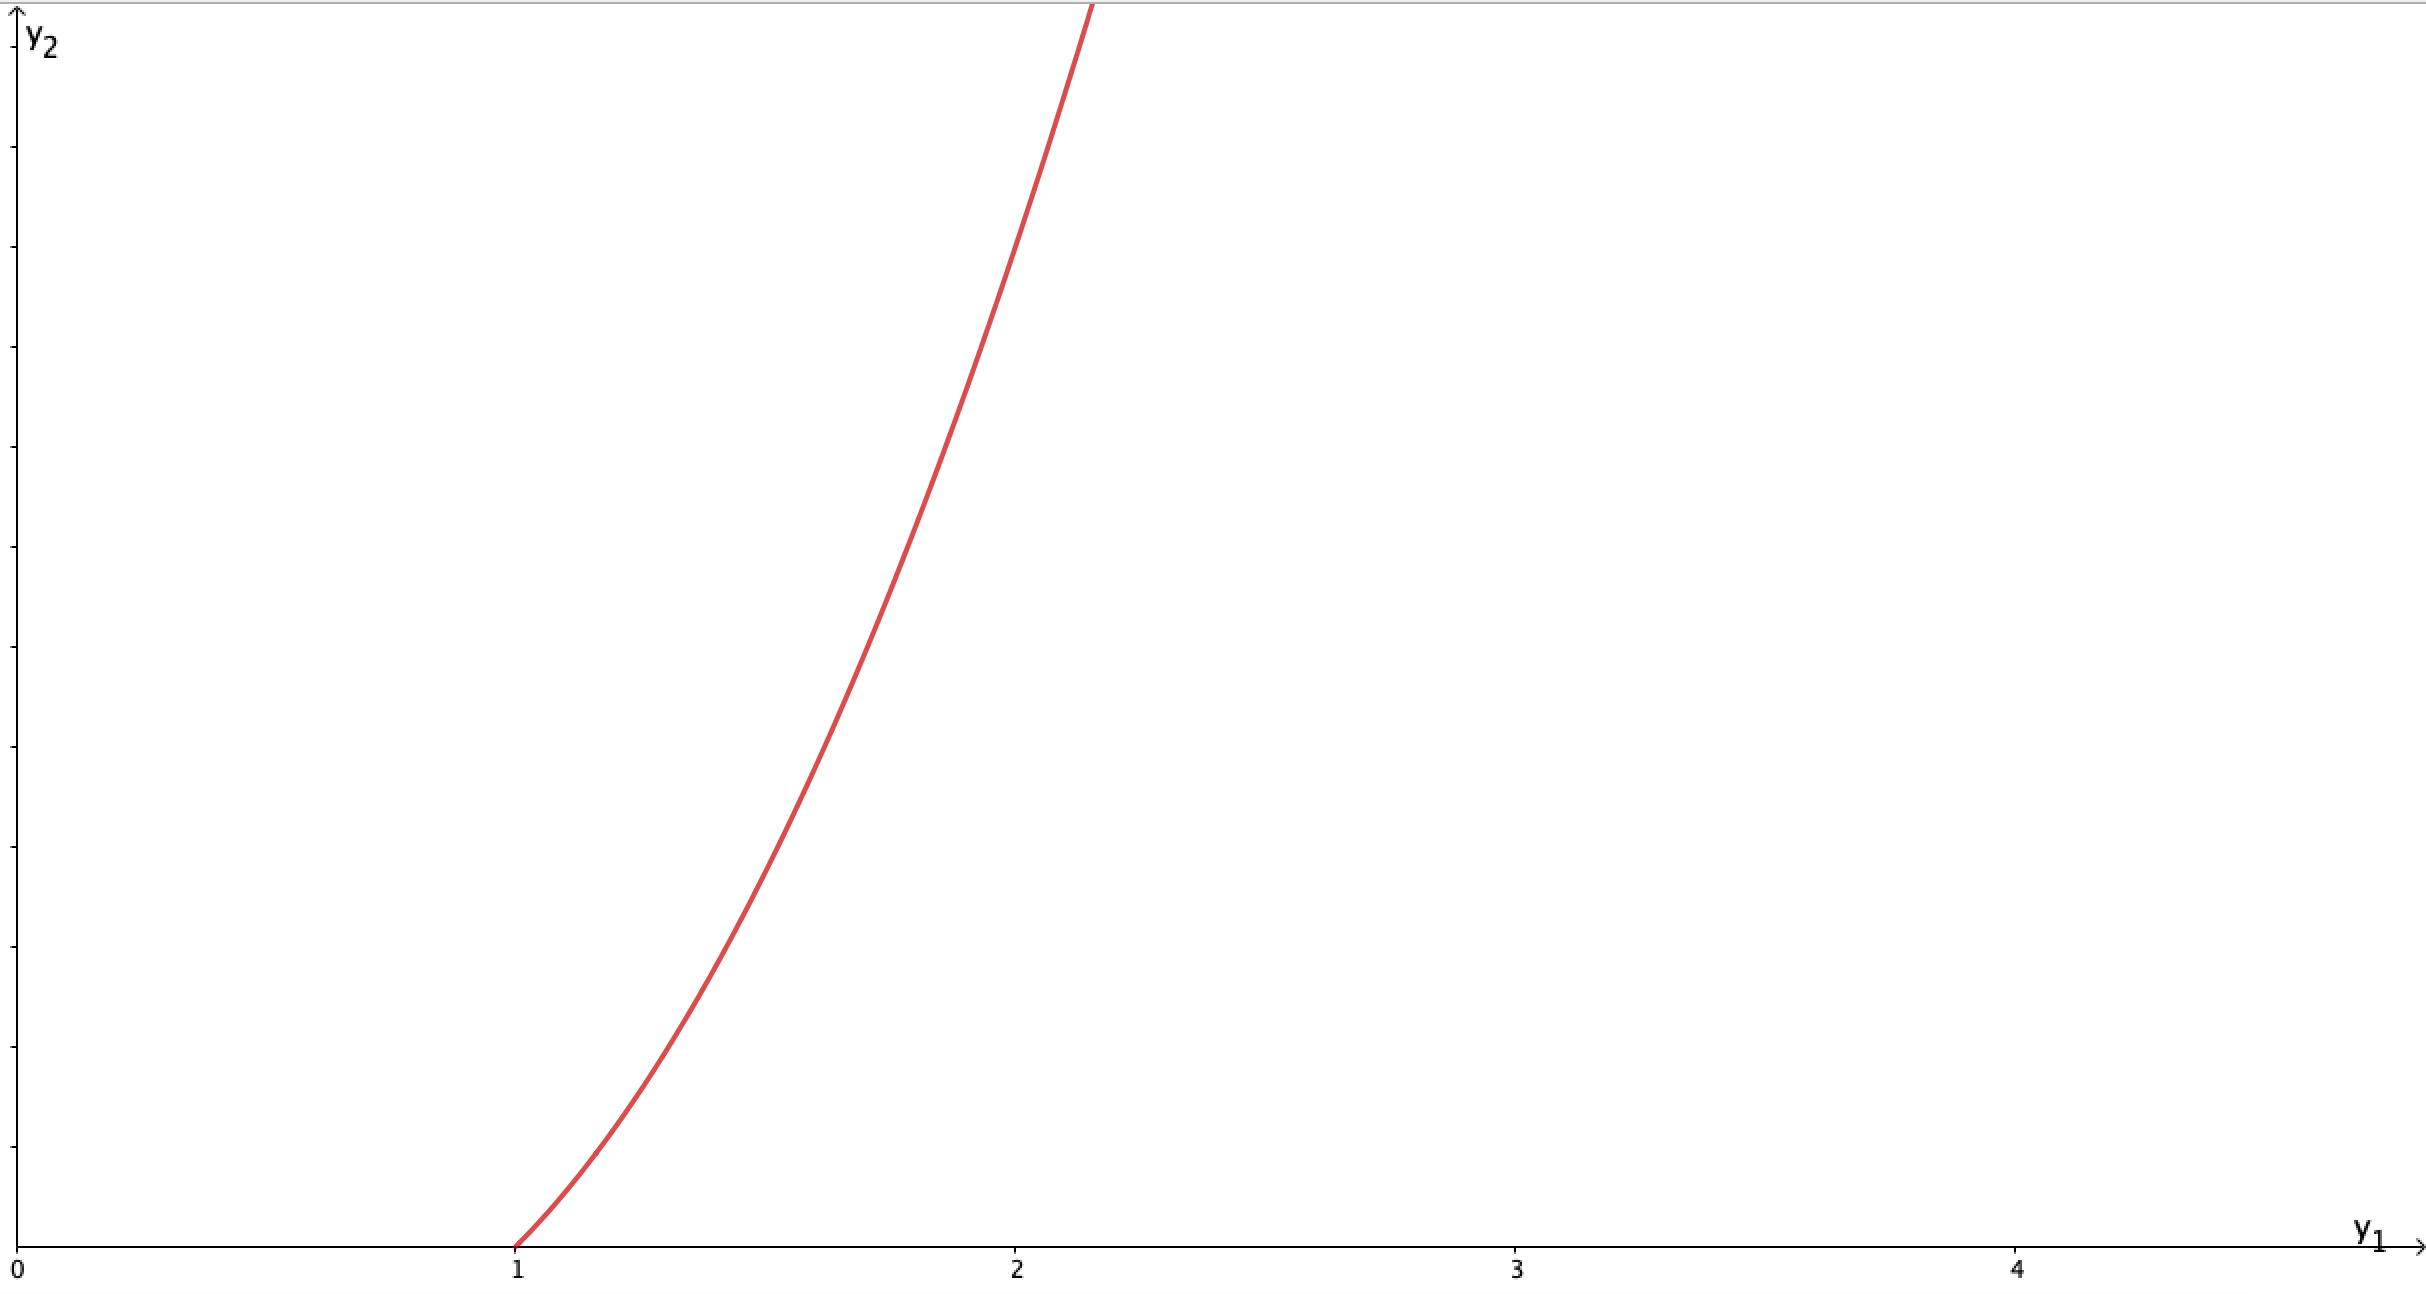
\includegraphics[width=0.5\linewidth]{./figures/e16_3.png}
  \caption{}
  \label{fig:e16_3}
\end{figure}




\subsection*{4.} Solve the system of ODEs
\[ 
\Vec{y}'(t) = A \Vec{y}(t), A = \begin{pmatrix}
1 & 0\\
0 & 1\\
\end{pmatrix}
.\]
Determine the type of critical point at the origin of the phase plane and sketch the phase portrait around the critical point. Assume that $- \infty < t < \infty$.
\bigbreak
We start by finding the eigenvalues of $A$ as:
\[ 
  \mathrm{det}(A - \lambda I) = \left| \begin{array}{cc}
  1 - \lambda & 0\\
  0 & 1 - \lambda\\
  \end{array} \right| = \left( 1 - \lambda^2 \right) = 0
.\]
By the zero-rule we get that $\lambda_1 = \lambda_2 = 1$. We find the eigenvectors of these as:
\[ 
A \Vec{x} = \lambda \Vec{x} = \Vec{x} \implies \left( A - I \right) \Vec{x} = \Vec{0} \implies \begin{pmatrix}
0 & 0\\
0 & 0\\
\end{pmatrix} \begin{pmatrix}
x_1\\
x_2\\
\end{pmatrix} = \begin{pmatrix}
0\\
0\\
\end{pmatrix}
.\]
We can choose two linearly independent eigenvectors as:
\[ 
\Vec{x}^{(1)} = \begin{pmatrix}
1\\
0\\
\end{pmatrix}, \qquad \Vec{x}^{(2)} = \begin{pmatrix}
0\\
1\\
\end{pmatrix}
.\]
The general solution is therefore:
\[ 
\Vec{y}(t) = c_1 \Vec{x}^{(1)} e^{\lambda_1 t} + c_2 \Vec{x}^{(2)} e^{\lambda_2 t} = c_1 \begin{pmatrix}
1\\
0\\
\end{pmatrix} e^{t} + c_2 \begin{pmatrix}
0\\
1\\
\end{pmatrix}e^{t}
.\]
From this we see that:
\[ 
y_1(t) = c_1 e^{t}, \qquad y_2(t) = c_2 e^{t}
.\]
We now define:
\begin{align*}
  p &= \lambda_1 + \lambda_2 = 2 \\
  q &= \lambda_1 \lambda_2 = 1 \\
  \Delta &= \left( \lambda_1 - \lambda_2 \right)^2 = 0
.\end{align*}
This means there is an unstable node at $(0,0)$. Now we must examine where $\left( y_1, y_2 \right)$ is placed based on the values of $c_1$ and $c_2$ as:
\begin{itemize}
  \item For $c_1 = 0, c_2 \geq 0$: $(y_1, y_2)$ on positive $y_2$-axis
  \item For $c_1 = 0$, $c_2 <0$: On negative $y_2$-axis
  \item For $c_1 \geq 0$, $c_2 = 0$: On positive $y_1$-axis
  \item For $c_1 < 0$, $c_2 = 0$: On negative $y_1$-axis
\end{itemize}
We can also write $y_2$ in terms of $y_1$ as:
\[ 
y_2 = \frac{c_2}{c_1} y_1
.\]
A phase field can therefore be produced as shown on \textbf{\autoref{fig:e16_4}}
\begin{figure} [ht]
  \centering
  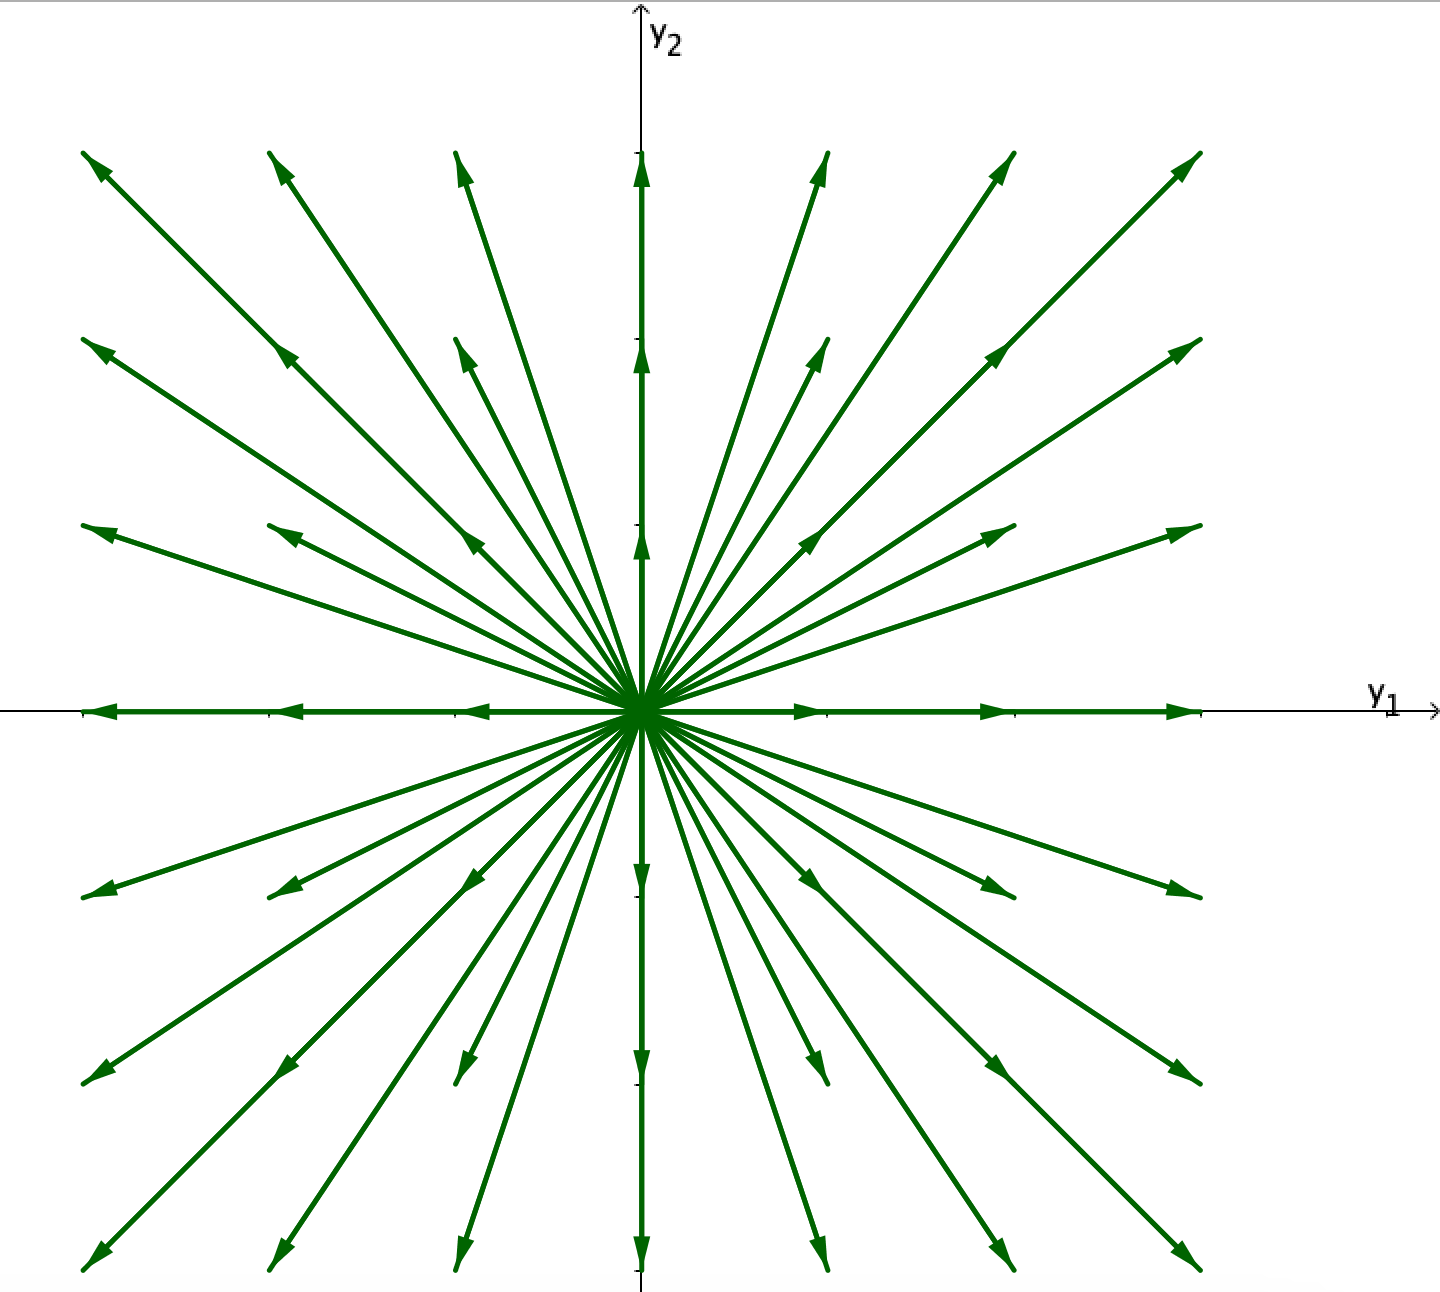
\includegraphics[width=0.5\linewidth]{./figures/e16_4.png}
  \caption{}
  \label{fig:e16_4}
\end{figure}





\subsection*{5.} Rewrite the ODE
\[ 
y''(t) - y'(t) - 2y(t) = 0
\]
as a system of 2 first order ODEs. Solve the system of ODEs. Determine the type of critical point at the origin of the phase plane and sketch the phase portrait around the critical point. Assume that $- \infty < t < \infty$.
\bigbreak
We define:
\[ 
y_1(t) = y(t), \qquad y_2(t) = y'(t)
.\]
And get the system of first order ODEs:
\begin{align*}
  y_1'(t) &= y_2(t) \\
  y_2'(t) &= 2y_1(t) + y_2(t)
.\end{align*}
Which can be written on vector form as:
\[ 
\Vec{y}'(t) = A \Vec{y}(t), \quad A = \begin{pmatrix}
0 & 1\\
2 & 1\\
\end{pmatrix}, \quad \Vec{y}(t) = \begin{pmatrix}
y_1(t)\\
y_2(t)\\
\end{pmatrix}, \quad \Vec{y}'(t) = \begin{pmatrix}
y_1'(t)\\
y_2'(t)\\
\end{pmatrix}
.\]
We can now find the eigenvalues of $A$ as:
\[ 
\mathrm{det}(A - \lambda I) = \left| \begin{array}{cc}
-\lambda & 1\\
2 & 1 - \lambda\\
\end{array} \right| = (-\lambda)(1-\lambda) - 2 = 0
.\]
Therefore we get $\lambda_1 = 2$, $\lambda_2 = -1$. 
First we find the eigenvector for $\lambda_1 = 2$ as:
\[ 
A \Vec{x}^{(1)} = 2 \Vec{x}^{(1)} \implies \left( A - 2 I \right) \Vec{x}^{(1)} = \Vec{0} \implies \begin{pmatrix}
-2 & 1\\
2 & -1\\
\end{pmatrix} \begin{pmatrix}
x_1^{(1)}\\
x_2^{(1)}\\
\end{pmatrix} = \Vec{0}
.\]
Here we choose $\Vec{x}^{(1)} = \begin{pmatrix}
1\\
2\\
\end{pmatrix}$. Now we can find the eigenvector for $\lambda_2 = -1$ as:
\[ 
A \Vec{x}^{(2)} = - \Vec{x}^{(2)} \implies \left( A + I \right) \Vec{x}^{(2)} = \Vec{0} \implies \begin{pmatrix}
  1 & 1\\
  2 & 2\\
\end{pmatrix} \begin{pmatrix}
x_1^{(1)}\\
x_2^{(1)}\\
\end{pmatrix} = \Vec{0}
.\]
Here we choose $\Vec{x}^{(2)} = \begin{pmatrix}
1\\
-1\\
\end{pmatrix}$. Therefore the general solution is:
\[ 
\Vec{y}(t) = \begin{pmatrix}
y_1(t)\\
y_2(t)\\
\end{pmatrix} = c_1 \Vec{x}^{(1)} e^{\lambda_1 t} + c_2 \Vec{x}^{(2)} e^{\lambda_2 t} = c_1 \begin{pmatrix}
1\\
2\\
\end{pmatrix} e^{2t} + c_2 \begin{pmatrix}
1\\
-1\\
\end{pmatrix} e^{-t}
.\]
Therefore we have:
\begin{align*}
  y_1(t) &= y(t) = c_1 e^{2t} + c_2 e^{-t} \\
  y_2(t) &= y'(t) = 2c_1 e^{2t} - c_2 e^{-t}
.\end{align*}
We can now define:
\begin{align*}
  p &= \lambda_1 + \lambda_2 = 1 \\
  q &= \lambda_1 \lambda_2 = -2 \\
  \Delta &= \left( \lambda_1 - \lambda_2 \right)^2 = 9
.\end{align*}
Therefore we have an unstable saddle point at $\left( 0,0 \right) $. Now we must examine the behavior of the functions around the saddle point as:
\begin{itemize}
  \item For $c_1 = 0, c_2 \neq 0$: $y_2 = -y_1$
  \item For $c_1 \neq 0, c_2 = 0$: $y_2 = 2y_1$
  \item For $c_1 \neq 0, c_2 \neq 0, t \to \infty$: $y_2 = 2y_1$
  \item For $c_1 \neq 0, c_2 \neq 0, t \to -\infty$: $y_2 = - y_1$
\end{itemize}
Now this can be plotted as shown on \textbf{\autoref{fig:e16_5}}.
\begin{figure} [ht]
  \centering
  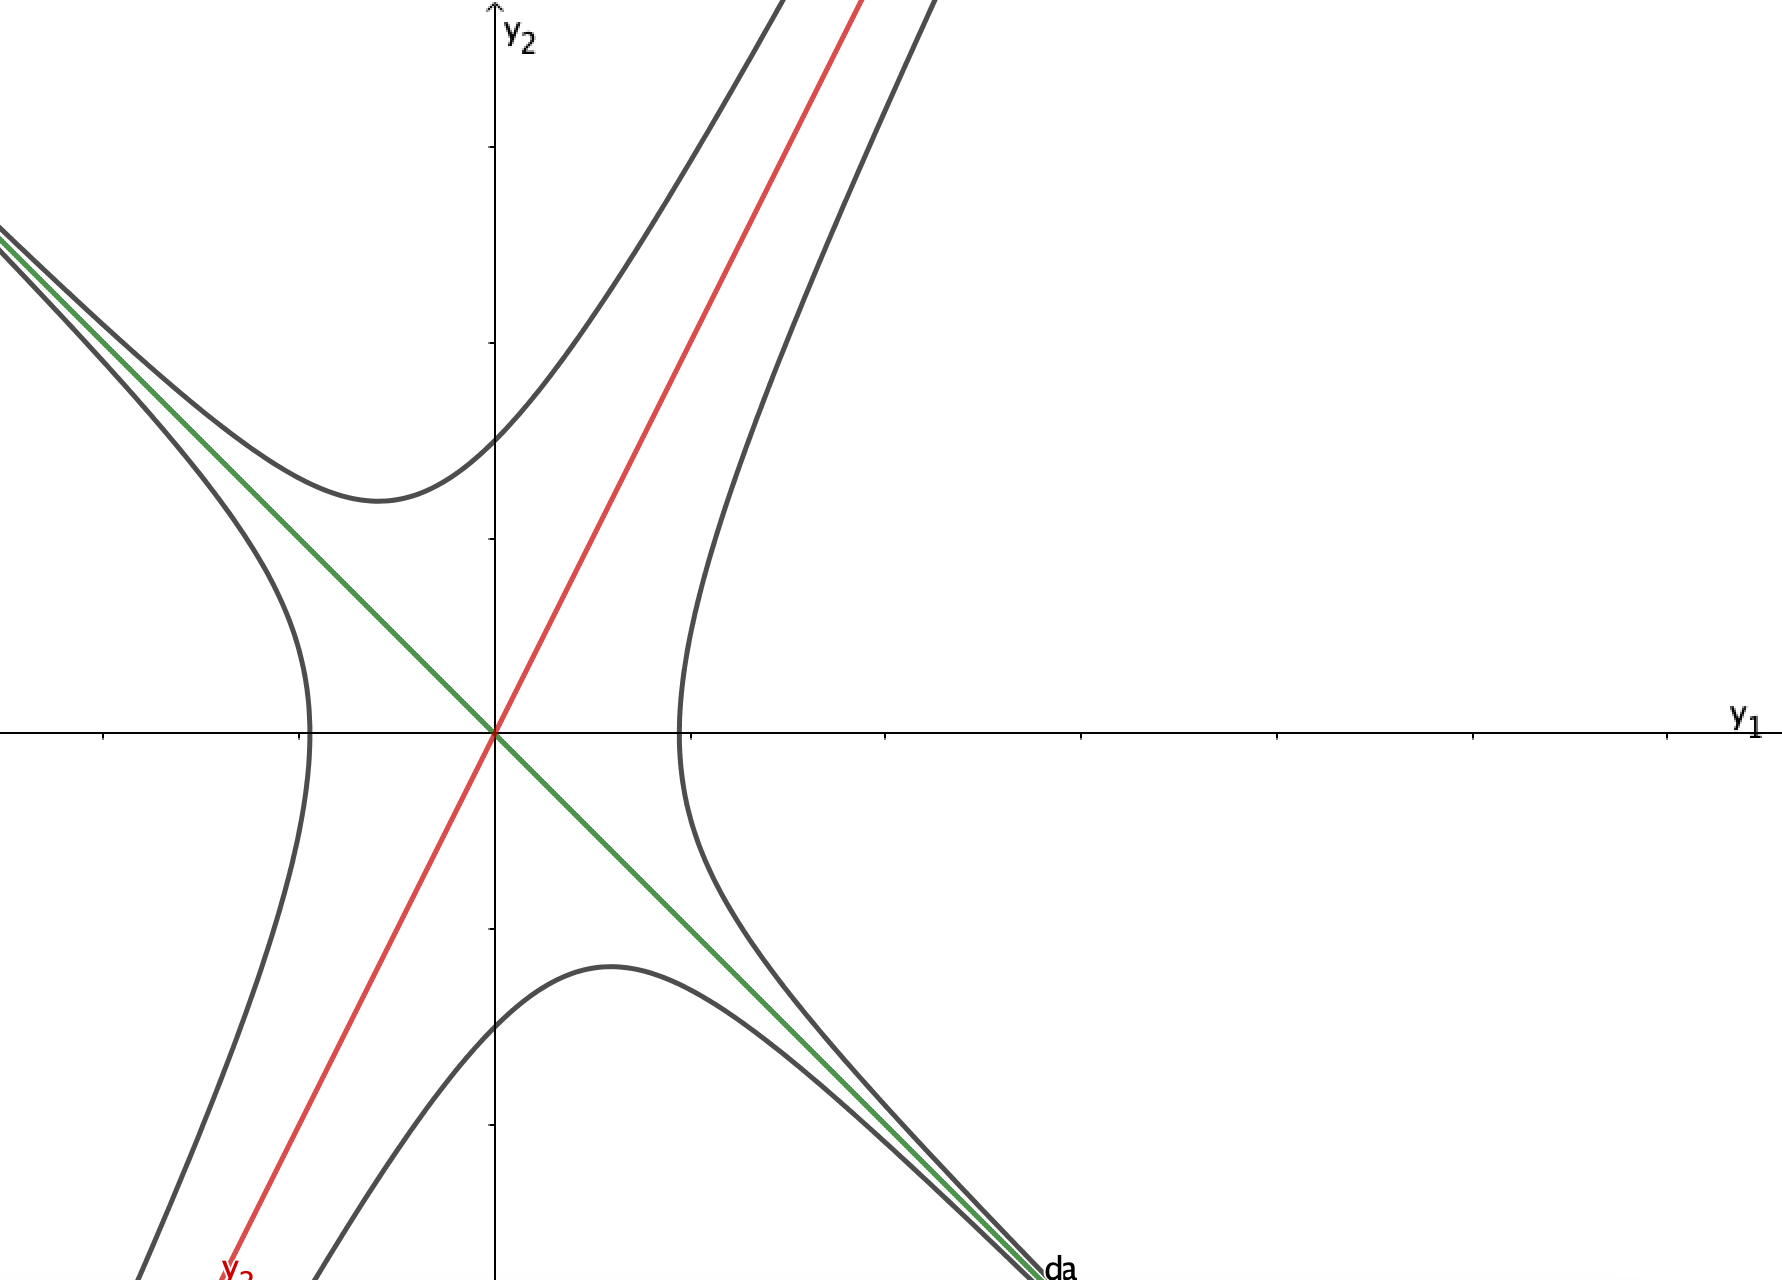
\includegraphics[width=0.5\linewidth]{./figures/e16_5.png}
  \caption{}
  \label{fig:e16_5}
\end{figure}
